\documentclass{article}
\usepackage{amsmath, amssymb, stmaryrd}
\usepackage{geometry}
\usepackage{graphicx}
\geometry{a4paper, margin=0.8in}


\begin{document}
\begin{center}
    {\large\textbf{IEOR 221 Assignment 9}}\\
    Group members: Haotian Lan, Hua-Shin Chang, Jiaming Camuseau
\end{center}

\noindent\textbf{1.} The following is the result from CRR tree under different number of steps. Vega and rho are computed by central finite differences with absolute bumps of $10^{-4}$.

\begin{center}
\textbf{CRR}\\[0.5em]
\begin{tabular}{rrrrrrr}
    \hline
    $N$ & NPV & Delta & Gamma & Theta & Vega & Rho \\
    \hline
    $2^{11}$ & 21.1236 & 0.5218 & 0.0060 & -1.0722 & 67.1493 & 85.1271 \\
    $2^{12}$ & 21.1245 & 0.5217 & 0.0060 & -1.0718 & 67.1536 & 85.1444 \\
    $2^{13}$ & 21.1249 & 0.5217 & 0.0060 & -1.0716 & 67.1550 & 85.1444 \\
    $2^{14}$ & 21.1251 & 0.5217 & 0.0060 & -1.0715 & 67.1557 & 85.1448 \\
    $2^{15}$ & 21.1252 & 0.5217 & 0.0060 & -1.0715 & 67.1561 & 85.1452 \\
    \hline
\end{tabular}
\end{center}

\indent For the accuracy of the result, we have to look into the asymptotic behavior of the $CRR$ tree.
First notice that for a payoff with enough smoothness, the price $V_N$ computed from CRR tree using $N$ steps has the asymptotic behavior
\begin{equation}
    V_N = V + \frac{C}{N} + o(N^{-1}), \label{CRR_asymptotic}
\end{equation}
where $C$ is a constant and $V$ is the true price of the option. In this case, if we let 
\[
    D_N = V_{2N} - V_N = -\frac{C}{2N} + o(N^{-1}),
\]
then
\[
    \lim_{N\to\infty}\frac{D_{2N}}{D_N} = 2 \qquad \lim_{N\to\infty} N\cdot D_N = -\frac{C}{2}
\]
However, the payoff of the option is not smooth at the strike $K$, and whether $K$ is in the ternimal price grids changes the value of $C$. Since the option is ATM, $K$ is in the ternimal price grids only when $N$ is even. So we have to separate this into cases where $N$ is even or odd. Plotting the graph of $D_{2N} / D_N$ (replace $2N$ by $2N+1$ in above formulas if $N$ is odd) and $N D_N$, we have the following.
\begin{center}
    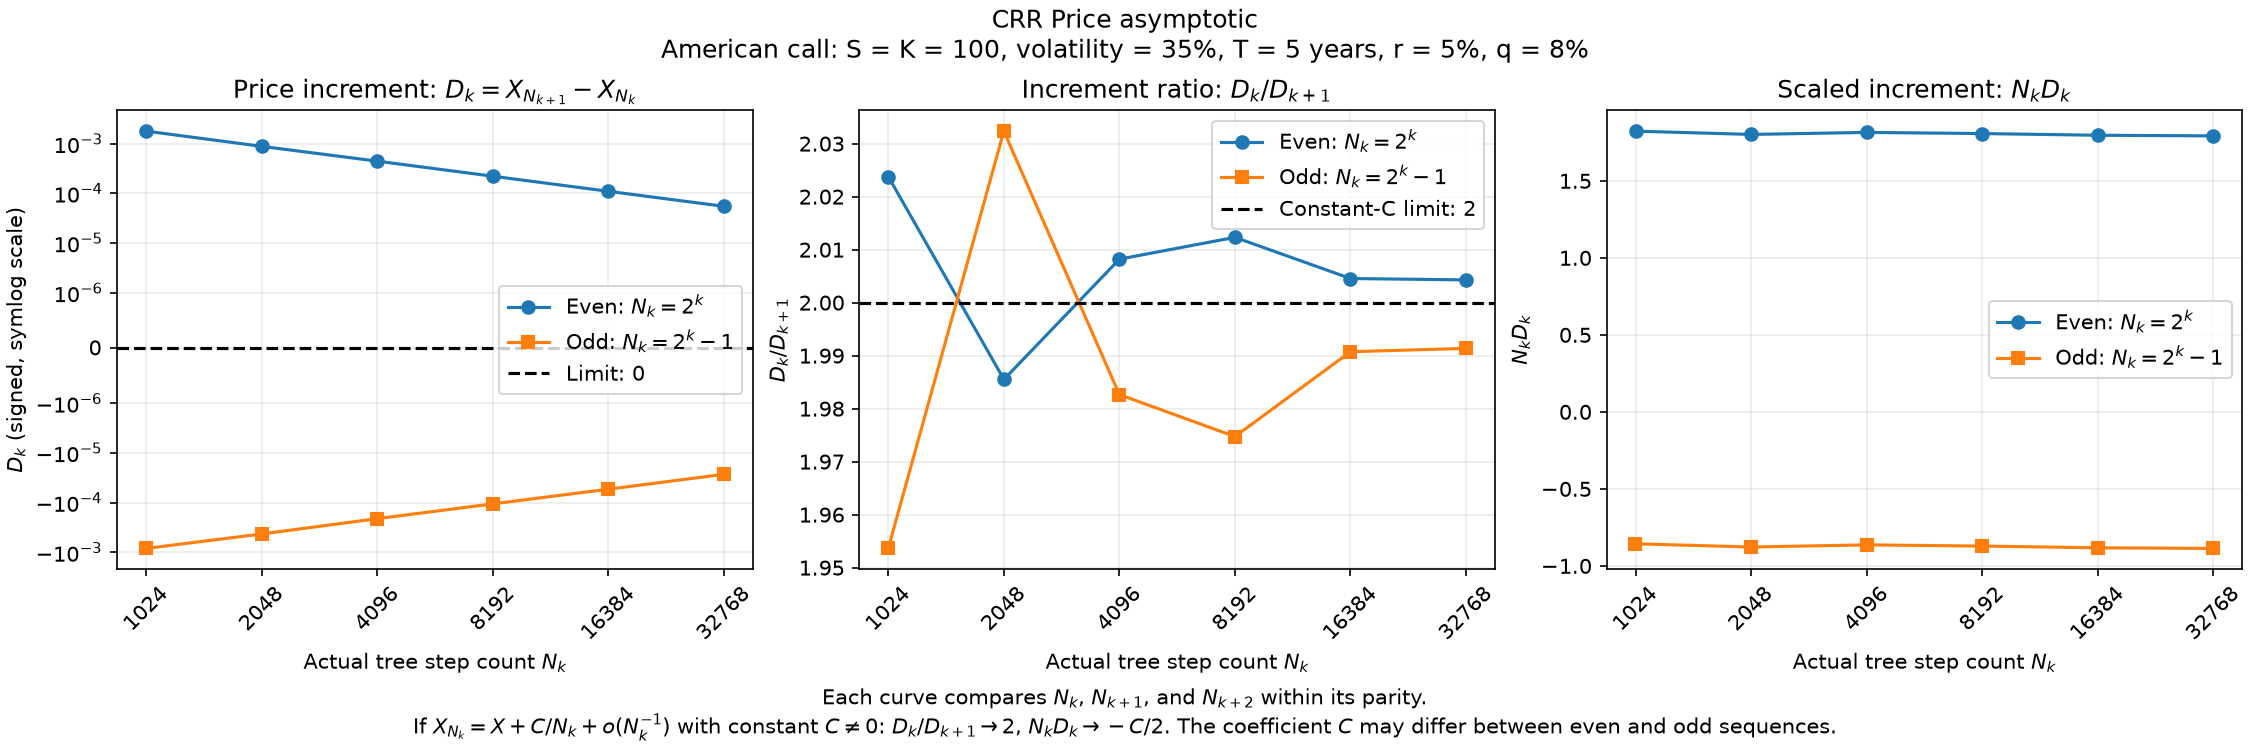
\includegraphics[width=\textwidth]{crr_asymptotic_price.png}
\end{center}
We can see that $V_N$ does follow a similar asymptotic behavior as (\ref{CRR_asymptotic}) for even and odd $N$, respectively, with $C_{even} \approx -3.52$ and $C_{odd} \approx 1.74$. Hence the error of the result at 32768 steps is approximately $-0.000107$, and the true price should be approximately $21.1253$.\\

\indent For the delta, gamma, and theta, we use the same error analysis to see that a similar asymptotic behavior as (\ref{CRR_asymptotic}) is satisfied, and get that delta, gamma, and theta are approximately 0.5217, 0.0060, and -1.0714, respectively.\\

\indent Finally, for vega and rho, we need to take acount the effect of the bump size $h$, which makes the analysis more complicated. From the tables, we can see that the accuracy for these two greeks are not enough for 4 decimal places.\\

We also use a BBSR tree to give another estimation of the price and greeks, which shows a better convergance behavior:

\begin{center}
\textbf{BBSR}\\[0.5em]
\begin{tabular}{rrrrrrr}
    \hline
    $N$ & NPV & Delta & Gamma & Theta & Vega & Rho \\
    \hline
    $2^{11}$ & 21.1254 & 0.5217 & 0.0060 & -1.0715 & 67.1584 & 85.1632 \\
    $2^{12}$ & 21.1254 & 0.5217 & 0.0060 & -1.0714 & 67.1564 & 85.1440 \\
    $2^{13}$ & 21.1253 & 0.5217 & 0.0060 & -1.0714 & 67.1564 & 85.1450 \\
    $2^{14}$ & 21.1253 & 0.5217 & 0.0060 & -1.0714 & 67.1565 & 85.1456 \\
    $2^{15}$ & 21.1253 & 0.5217 & 0.0060 & -1.0714 & 67.1565 & 85.1457 \\
    \hline
\end{tabular}
\end{center}

\medskip
\noindent\textbf{2.} For the antithentic method, we used the opposite-sign normal samples as a pair. 
For the control variate method, we implemented two different control functions, 
which are the ternimal stock price and the price of corresponding geometric Asian call option.

\begin{center}
\begin{tabular}{lrr}
    \hline
    Method & NPV & MC standard error \\
    \hline
    Plain MC & 5.1914 & 0.0085 \\
    Control variate (terminal stock price) & 5.1932 & 0.0057 \\
    Control variate (geometric Asian call) & 5.1984 & 0.0003 \\
    Antithetic MC & 5.1966 & 0.0069 \\
    Antithetic + control variate (terminal stock price) & 5.1981 & 0.0049 \\
    Antithetic + control variate (geometric Asian call) & 5.1987 & 0.0003 \\
    \hline
\end{tabular}
\end{center}

\noindent Each method uses $2^{20}$ simulated paths, the fixed seed $0$, and is computed on CUDA. For antithetic methods, these paths form $2^{19}$ pairs. Using the result from CV with geometric asian option, we have the 95\% CI is [5.1978, 5.1992]. When rounding to 2 decimal places, the price is approximately 5.20.\\
 
The price of the vanilla call option with the same strike and maturity is $8.8249$. The reason why it's higher that the price of the Asian optnio is that the average of prices have a lower variance than that of the ternimal stock price. Although $q > r$ makes the expected value of the average of prices slightly higher that than that of the ternimal price, its effect on the option price is relative small compare to the effect of the difference of variance, hence gives a lower price for Asian option. 
\end{document}
